\documentclass[12pt,letterpaper]{article}

% Shared manuscript formatting for the generic arXiv build.
\usepackage[letterpaper,margin=1in]{geometry}
\usepackage[T1]{fontenc}
\usepackage[utf8]{inputenc}
\usepackage{lmodern}
\usepackage{microtype}
\usepackage{amsmath}
\usepackage{amssymb}
\usepackage{graphicx}
\usepackage{xcolor}
\usepackage{soul}
\usepackage[normalem]{ulem}
\usepackage{xspace}
\usepackage{placeins}
\usepackage{caption}
\usepackage{lineno}
\usepackage[numbers,sort&compress]{natbib}
\usepackage{hyperref}
\usepackage{xurl}
\usepackage[capitalise,nameinlink]{cleveref}

\hypersetup{
  colorlinks=true,
  linkcolor=blue,
  citecolor=blue,
  urlcolor=blue,
  pdfauthor={Emily Howerton et al.},
  pdftitle={Dynamic consequences of declining vaccination coverage in a heterogeneous world}
}

% Light-grey continuous line numbers for collaborative review.
\definecolor{linenogray}{gray}{0.65}
\renewcommand{\linenumberfont}{\normalfont\tiny\sffamily\color{linenogray}}

% Author comments in David's usual bracketed style.
\definecolor{commentorange}{RGB}{210,105,0}
\definecolor{commentblue}{RGB}{40,80,180}
\newcommand{\commentmacro}{\showcomment}
\newcommand{\showcomment}[3]{\textcolor{#1}{\textbf{[#2: }\textsl{#3}\textbf{]}}}
\newcommand{\nocomment}[3]{}
\newcommand{\david}[1]{\commentmacro{cyan}{David}{#1}}
\newcommand{\emily}[1]{\commentmacro{magenta}{Emily}{#1}}
\newcommand{\jess}[1]{\commentmacro{commentorange}{Jess}{#1}}
\newcommand{\bryan}[1]{\commentmacro{commentblue}{Bryan}{#1}}
\newcommand{\dsugg}[1]{{\color{red}#1}}
\newcommand{\stkout}[1]{{\color{blue}\ifmmode\text{\sout{\ensuremath{#1}}}\else\sout{#1}\fi}}
\newcommand{\thickredline}{\par\bigskip\noindent{\color{red}\rule{\linewidth}{4pt}}\par\bigskip}

% Reproduction-number and vaccination notation.
\newcommand{\R}{\mathcal{R}}
\newcommand{\Rn}{\R_{0}}
\newcommand{\Reff}{\R_{\mathrm{eff}}}
\newcommand{\vcrit}{v_{\mathrm{crit}}}

% Frequently used prose and calculus macros.
\newcommand{\ie}{\textit{i.e., }}
\newcommand{\eg}{\textit{e.g., }}
\newcommand{\etc}{\emph{etc.}\xspace}
\newcommand{\dee}{\mathrm{d}}
\newcommand{\dd}[2]{\frac{\dee #1}{\dee #2}}

\captionsetup{font=small,labelfont=bf}
\setlength{\parindent}{1.5em}
\setlength{\parskip}{0pt}

% Keep review comments out of the PDF bookmarks and metadata strings.
\pdfstringdefDisableCommands{%
  \def\david#1{}%
  \def\emily#1{}%
  \def\jess#1{}%
  \def\bryan#1{}%
  \def\dsugg#1{#1}%
  \def\stkout#1{}%
}


\title{\textbf{Dynamic consequences of declining vaccination coverage in a heterogeneous world}}
\author{%
  Emily Howerton\textsuperscript{1,*},
  Ayesha Mahmud\textsuperscript{2},
  David \dsugg{J.\,D. }Earn\textsuperscript{3},\\
  Bryan T. Grenfell\textsuperscript{1},
  C. Jessica E. Metcalf\textsuperscript{1}\\[0.8em]
  \small \textsuperscript{1}Department of Ecology and Evolutionary Biology, Princeton University\\
  \small \textsuperscript{2}Department of Demography, University of California, Berkeley\\
  \small \textsuperscript{3}Department of Mathematics and Statistics, McMaster University\\[0.5em]
  \small *Corresponding author: \href{mailto:ehowerton@princeton.edu}{ehowerton@princeton.edu}
}
\date{}

\begin{document}

\maketitle
\linenumbers

\noindent\emily{David, let us know what you think. Please feel free to
add comments throughout.}

\begin{abstract}
The current landscape of global health suggests the possibility of rapid
declines in vaccination coverage, potentially compounding the slow
declines that have been observed in a number of countries across the
globe. Rich theory has been developed to evaluate the consequences of
increases in vaccination coverage including counterintuitive outcomes
such as the honeymoon effect, where low levels of transmission are
observed despite sub-optimal coverage. Yet, the consequences of reverses
in global vaccination coverage have been less explored, especially where
they may interact with honeymoon dynamics. While equilibrium analyses
support the intuition that following vaccine reduction, the eventual
onset of major epidemics is inevitable, in practice, major outbreaks
seemingly occur after a longer honeymoon period than would be predicted
by standard theory. Here, we present a theoretical framework for
understanding how honeymoon dynamics interact with declining vaccination
coverage. We show that the eventual return of vaccine preventable
outbreaks could be slower than we might expect, given that the
accumulation of susceptible individuals through new births is expected
to be a gradual process, especially in places where coverage declines
are modest or incremental. Moreover, situating a single under-vaccinated
community in a broader network of vaccinated \stkout{places}\dsugg{populations}
could potentially serve as an additional
buffer, but more detailed network theory is needed. Nevertheless, when
an importation hits a pool of susceptible individuals, age-structured
\david{Do you mean age-structured contact patterns? i.e., the contact
rate is much higher in schoolchildren than adults?}dynamics could make
the outbreak even more explosive\david{More explosive than what? than it
would be in a homogeneously mixed population?}. Prevailing uncertainties
around vaccination coverage and the history of infection make detailed
serology in key social groups a vital component to measure susceptibility
and predict risk of subsequent outbreaks.
\end{abstract}

\section{Introduction}
\label{sec:introduction}

The increase of vaccination coverage has been a triumph of global health, estimated to have averted millions of deaths in the last 30 years \citep{ToorEtAl2021}. Welcome advances in vaccine technology mean that many more vaccines are nearing deployment. Yet, vaccination gains are currently under threat given a shifting political landscape and increasing vaccine hesitancy \citep{OliveEtAl2018}.

A key exemplar of the power of vaccines is the success of measles vaccination. Measles vaccination has been called a best buy in public health as a result of the low cost of the vaccine, and the potentially high case fatality rate of the infection, whether directly \citep{PortnoyEtAl2019}, associated with secondary infections \citep{XiaEtAl2023}, or in the longer term as a result of `immune amnesia' \citep{MinaEtAl2015}. The introduction of the measles vaccine has resulted in vast gains in life saved around the world \citep{ToorEtAl2021}.

In the absence of vaccination, drivers of measles dynamics are well understood. Birth rates drive the replenishment of susceptibles to fuel outbreaks. If the number of susceptible individuals is sufficient, there are additional factors that regulate when outbreaks occur, such as seasonality in transmission (e.g., from school calendars) \citep{FineClarkson1982,BjornstadEtAl2002}, stochasticity \citep{Bartlett1960}, and connectivity and community size \citep{BjornstadGrenfell2008}. Together, these factors determine the periodicity of outbreaks, from outbreaks that occur annually to chaotic dynamics that are in principle unpredictable \citep{FerrariEtAl2008,DalzielEtAl2016}.

Dramatic changes in outbreak dynamics can result from the introduction of vaccination. By effectively reducing the supply rate of susceptibles, vaccination can drive measles away from the seasonal annual or multi-annual attractor in ways that may result in long transient periods. Incidence typically decreases steadily as coverage increases, but outbreaks also become more sporadic and less predictably timed \citep{GrahamEtAl2019}. Notably, large outbreaks can even occur following years of (apparently) successful control, a phenomenon termed a ``post honeymoon period'' outbreak \citep{McLeanAnderson1988}, for which signatures can be detected in historical measles dynamics of countries across the world \citep{MetcalfEtAl2020}.

The equally important but opposite question of how dynamics change as vaccination declines \citep[e.g.,][]{BauchEarn2004} has been much less explored. Despite tremendous gains in vaccination coverage over the last forty years, there are also an increasing number of countries around the world that have experienced both rapid and gradual declines in coverage (Figure \ref{fig:global-coverage}). One recent study estimated that 8-10\% of school-age children in the US had missed at least one dose of the measles, mumps, and rubella vaccine \citep[for states where data was available]{ChenBento2026}. The consequences of such declines are also becoming increasingly clear, as measles outbreaks continue to strike across the globe \citep{DoMulholland2025}. Yet, \stkout{initially, these outbreaks seem to be less explosive}\dsugg{thus far, we have seen measles outbreaks in far fewer places}\david{Is there a reference that can be cited to support this statement?} \jess{it does feel a bit funny to have no evidence for this central claim?}\jess{but just as for the above... not quite sure what the evidence we bring to bear is---London having had $<90\%$ coverage for years and years? Things like that?}\emily{Yes, this is a good point... what do you think about this reframing where we just note the discrepancy between places with low coverage and places where an outbreak has occurred?}\emily{Bryan also suggested to emphasize this as a mystery when we discuss network dynamics in the Discussion (I will add this)} than would be predicted by standard epidemiological theory. Why could this be? Are there forces that could be slowing measles resurgences in the context of declining vaccination?

Here, we address this question through the lens of the epidemiological ``honeymoon''. We build upon standard theory on post-outbreak honeymoon dynamics to understand the dynamical consequences of declining vaccination coverage. We explore known drivers of honeymoon dynamics and extend the theory to include the role of age structure. We use these results as a foundation to interpret the current landscape of reported vaccination coverage. Together, this work provides a framework that can bound our expectations for future outbreak dynamics and help guide planning to avoid resurgent measles outbreaks in the future. Ascertainment of susceptible dynamics through serology emerges as a key priority.

\begin{figure}[p]
\centering
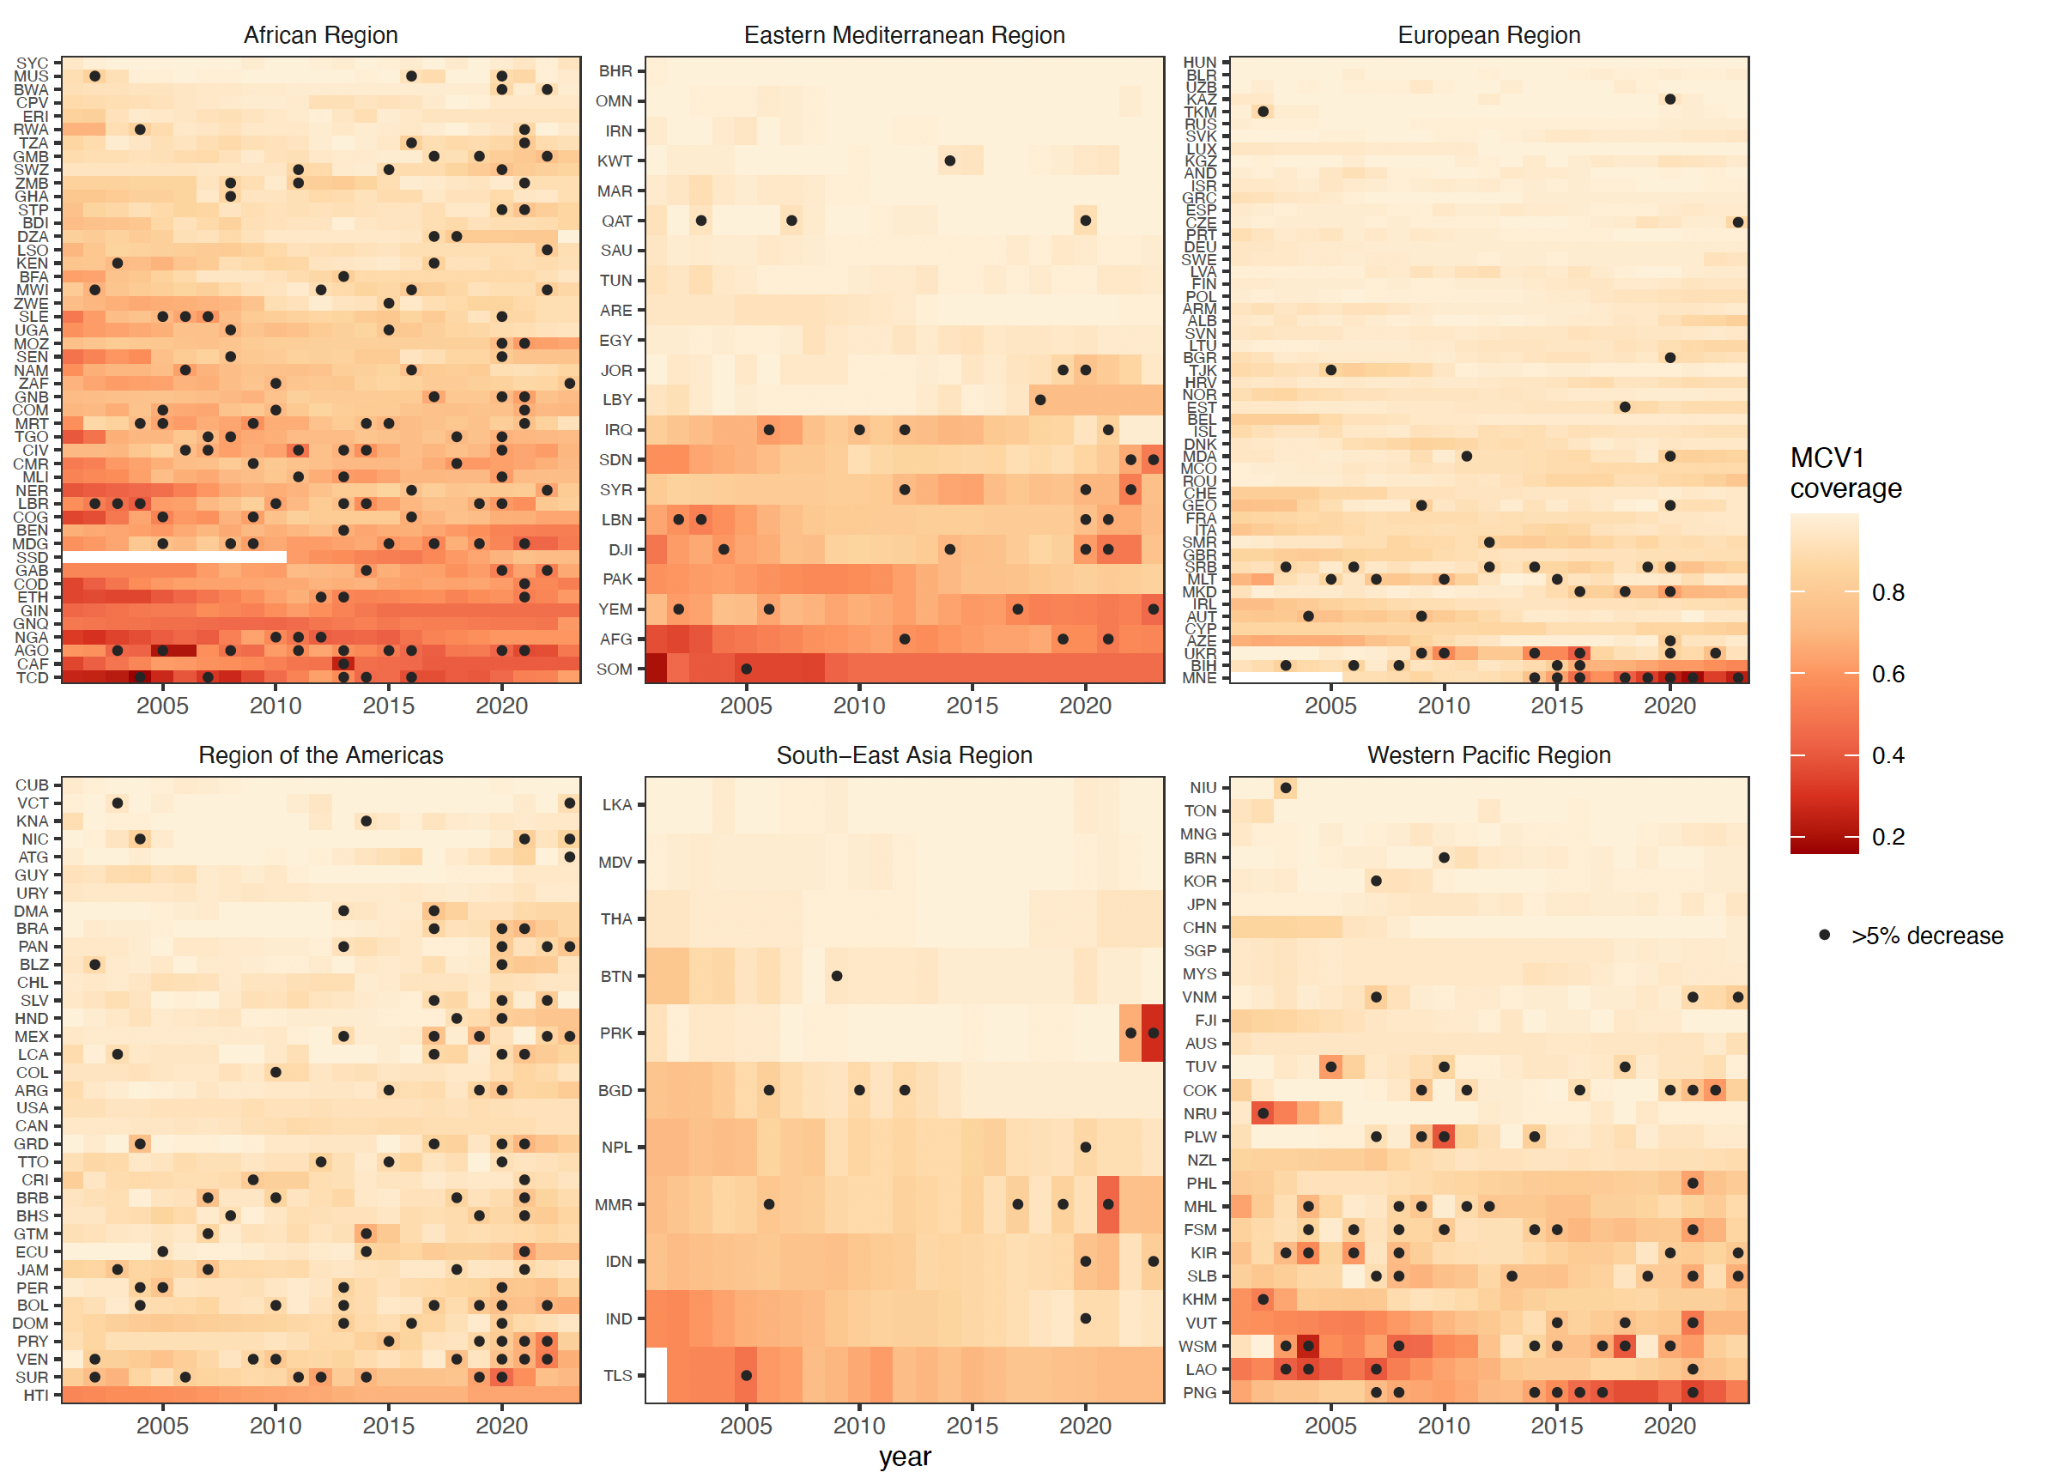
\includegraphics[width=\textwidth]{figures/figure1_global_mcv1_coverage.png}
\caption{\textbf{Reported first-dose coverage of measles containing vaccine (MCV1) across 195 countries from 2000--2023.} For each World Health Organization region, reported MCV1 coverage is shown for each year (darker red indicates lower coverage). Years where coverage decreased by at least 5\% (e.g., 95\% to 90\%, or 90\% to 75\%) are highlighted with a black dot. White indicates data \stkout{was}\dsugg{were} not available for that country and year. MCV1 data are collected from \citep{WHO_UNICEF2024}.}
\label{fig:global-coverage}
\end{figure}

\section{Modeling honeymoon dynamics under vaccination decline}
\label{sec:modeling-honeymoon}

A post-honeymoon outbreak requires the growth of a pocket of susceptible individuals that becomes large enough to fuel an outbreak (e.g., an age group missed by previous vaccination campaigns) and an imported infection to spark the outbreak. These two factors together contribute to the duration of the honeymoon period, where slower accumulation of susceptibles and lower importation rates lead to longer honeymoon periods \citep{McLeanAnderson1988,MetcalfEtAl2020}.

We hypothesize that these forces will also be key drivers if vaccination declines, although they may need to be recontextualized. While still replenished by birth rates, population-level susceptibility will depend on past infections, prior vaccination rates, and the extent of vaccination declines. Importation rates will be driven by connectivity with other communities and the prevalence of outbreaks among those connected communities.

While importation can be modeled deterministically, it is inherently a stochastic process that is difficult to predict. For this reason, we use the accumulation of susceptible individuals as the key marker of theoretical honeymoon times. In line with previous serologically based predictions of outbreaks \citep{ChenEtAl1990,GayEtAl1995,WinterEtAl2018,MetcalfEtAl2020}, the rate of susceptible accumulation determines the time until which an importation would successfully lead to an outbreak (on average) \citep{BjornstadEtAl2002}. In epidemiological theory\dsugg{, ignoring stochastic effects,} this time is the point at which the effective reproduction number exceeds one.

\section{Predictions from simple epidemiological theory}
\label{sec:simple-theory}

This definition of theoretical honeymoon time is analytically tractable in the Susceptible-Infected-Recovered (SIR) model of epidemiological dynamics. We model a population in which (1) measles is locally eliminated, and (2) susceptibility at the start of our analysis is determined by some pre-decline immunization level, which accounts for both vaccine coverage and efficacy.

For tractability, we opted for the simplest assumptions about how vaccination would decline: immunization drops immediately to a new level and remains there indefinitely. We call this ``post-decline immunization''. While in reality vaccination coverage fluctuates and changes in more complicated patterns, all such declines lead to an accumulation of susceptibles that is slower than immediately dropping to the lowest level. Thus, this simple assumption provides a worst-case scenario and a lower bound on the honeymoon period.

We can derive the theoretical honeymoon time, or the time until the effective reproduction number exceeds one, as

\david{I think it is better to write equations in a manifestly positive way: flip the fractions and get rid of the minus signs, since the negatives cancel.}

\begin{equation}
\begin{aligned}
  \text{theoretical honeymoon time} 
    &= -\frac{1}{\mu}\log\!\left( \frac{1/\Rn-(1-v)}{S_0-(1-v)} \right) \\ 
    &= \frac{1}{\mu}\log\!\left( \frac{S_v-S^*}{S_v-S_0} \right).
\end{aligned}
\label{eq:honeymoon-time-main}
\end{equation}

where $\mu$ is the birth and death rate, $\Rn$ is the basic reproduction number, $S_0$ is the proportion of the population susceptible before vaccination decline and $v$ is the post-decline rate of immunization \david{v is technically a proportion not a rate (similar to the logic of calling $R_0$ a number rather than a rate)}.

This formula can be easily interpreted. The term $S^* = 1/\Rn$ is the population-level susceptibility at which the model predicts the effective reproduction number is equal to one, and $S_{v}\  = 1 - v$ is the new susceptibility expected post-decline (in the absence of an outbreak). The ratio, then, describes the ``buffer'' of existing immunity that can be lost before the effective reproduction number exceeds one. Finally, $\frac{1}{\mu}$ characterizes how quickly these susceptibles will accumulate through births.

Honeymoon times are predicted to vary substantially, depending on the extent of immunization decline (Figure \ref{fig:simple-honeymoon}A, shown for a population with a life expectancy of 80 years and thus $\mu = 1/80$ years\textsuperscript{-1} and a pathogen like measles with $\Rn = 17$). When declines are dramatic, honeymoon times can be short (for example, less than a year if prior immunization levels are just above the herd immunity threshold). However, when declines are small, honeymoon times are predicted to be on the order of decades. For example, if the pre-decline immunization level is 96\%, honeymoon times are expected to be greater than 10 years as long as immunization does not drop below 80\%. Prior immunity in the population also has a substantial effect on honeymoon times; if pre-decline immunization is 95\% (instead of 96\%), a drop to 80\% immunization will yield a honeymoon time of 4.85 years.

We can also derive \david{again, refer to supp?} the relationship between pre-decline immunization, $v_0$, post-decline immunization, $v$, and theoretical honeymoon time, $t^H$:

\begin{equation}
v_0 = e^{\mu t^H}(1-1/\Rn)+(1-e^{\mu t^H})v.
\label{eq:coverage-isocline-main}
\end{equation}

We note a linear relationship between pre- and post-decline vaccination coverage, where birth rates modulate the slope and intercept of this relationship (Figure \ref{fig:simple-honeymoon}B). This suggests a simple conversion between pre-decline and post-decline immunization levels in terms of honeymoon time. Full derivations are provided in the Supplementary Material.\david{Ok. Consider flagging this earlier.}

\begin{figure}[p]
\centering
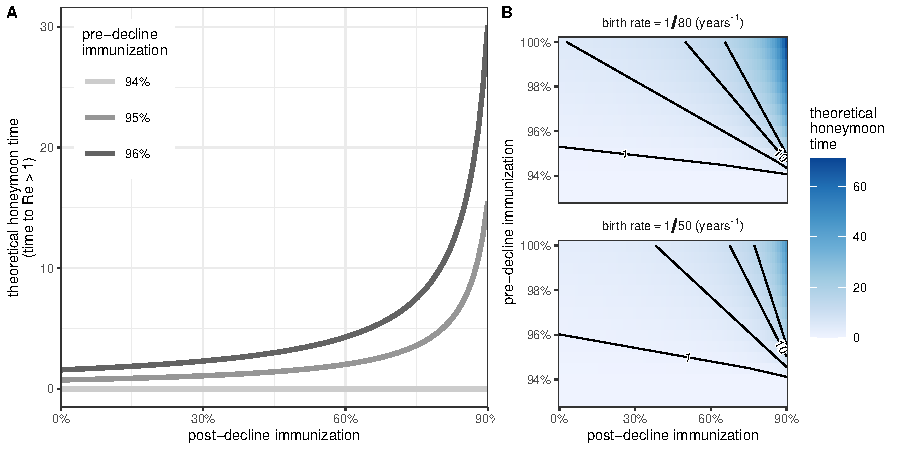
\includegraphics[width=\textwidth]{../figures/honeymoon_SIR_with_linear_heatmap.pdf}
\caption{\textbf{Theoretical honeymoon time predictions from basic epidemiological theory.} (A) Theoretical honeymoon time, computed as time until $\Reff>1$, by post-decline vaccination coverage. Three pre-decline immunization levels are shown (96\%: dark gray, 95\%: gray, 94\%: light gray). Results are shown for a population with $\mu = 1/80$ years\textsuperscript{-1} and a pathogen with $\Rn = 17$. (B) Relationship between pre- and post-decline immunization levels in a population with a slower birth rate (top, $\mu = 1/80$ years\textsuperscript{-1}) versus a faster birth rate (bottom, $\mu = 1/50$ years\textsuperscript{-1}). Again, we assume $\Rn = 17$.}
\label{fig:simple-honeymoon}
\end{figure}

\section{The effects of age structure on honeymoon times}
\label{sec:age-structure}

All of these theoretical predictions hinge on the assumption of a homogeneous population, where any individual is equally likely to contact all others. However, we know that heterogeneities in contact and transmission can have meaningful effects on dynamics, and one of the most important heterogeneities is related to age. Measles infection typically occurs when children first attend school or pre-school and first come into contact with large numbers of their peers \citep{FineClarkson1982}. This effect is likely to be particularly important in defining the delays to major outbreaks and associated transient dynamics as vaccination declines.

To explore the effects of age structure on honeymoon times, we leveraged a large body of previous work \citep{Schenzle1985}\david{Schenzle 1984 would be sensible to cite here too} to extend the basic SIR model to include age structure (see Methods for equations). The primary engine of this model is the WAIFW (who acquires infection from whom) matrix \citep{GrenfellAnderson1989,AndersonMay1991}, that describes transmission between individuals of different ages. Here we explore the extent to which the structure of the WAIFW matrix affects theoretical honeymoon times.

We tested five WAIFW matrices that span a range of contact-heterogeneity possibilities, (1) a \ul{flat} matrix, where contacts are equivalent across all age groups (equivalent to the homogeneous SIR model described in the previous section); (2) an empirically grounded matrix derived from the \ul{POLYMOD} contact surveys \citep{MossongEtAl2008}; and three synthetic matrices where (3) contacts are most intense among children along the \ul{diagonal} (i.e., among individuals of similar ages), and (4 and 5) where contacts \ul{peak at age 5} or \ul{peak at age 10} and minimal contacts among other age groups. Each WAIFW matrix is shown in Figure 3A. We assumed a stable age distribution at the start of vaccination decline and that birth and death rates were equivalent and constant over all ages. We also rescaled transmission rates across WAIFW matrices to ensure the same basic reproduction number in all cases. See Methods for details.

To get a sense for how age-structure affects transient outbreaks dynamics, we simulated outbreaks in a population that has experienced a significant decline in immunization to 20\% (again with $\Rn = 17$ and $\mu = 1/80$ years\textsuperscript{-1}, Figure \ref{fig:age-structured-outbreaks}). For simplicity, we introduced an infection into the population at the same time as immunization declines, but infection will remain at low levels until the effective reproduction number exceeds one (Figure \ref{fig:age-structured-outbreaks}B). In this example, the specifics of age-structured mixing patterns affect theoretical honeymoon times (i.e., when $\Reff$ crosses 1). Age structure can induce an earlier or similar timing of post-honeymoon outbreak compared to the homogeneous case (earlier: diagonal, similar: POLYMOD and peak at age 5), and some age structures can even delay post-honeymoon outbreaks. In the case of contacts that peak at age 10, new susceptibles must accumulate for years until they reach an age at which large scale transmission can occur (Figure \ref{fig:age-structured-outbreaks}D).

The intensity of post-honeymoon outbreaks also appears to depend on age structure (Figure \ref{fig:age-structured-outbreaks}C). To quantitatively compare these outbreaks, we used the unity beta calculation \citep{EarnEtAl2000,Mahmud2017,Bjornstad2018}\david{Do any of these sources use the term ``unity beta'' or present the argument? It was critical to the development of the 2000 paper, but I believe we left it out in the paper itself since it wasn't strictly necessary (no such thing as supp in 2000!).}. The unity beta \stkout{calculation} is a time-varying scalar that shows how age-structured outbreak dynamics (or dynamics with \stkout{any other population structure}\dsugg{associated with other population structures}) \stkout{can be simplified to be equivalent to dynamics}\dsugg{can be understood heuristically via the dynamical equations for aggregate variables (all susceptibles, all infectives, etc.), as} in the homogeneous case. For a model with $A$ discrete age classes, a transmission rate $\beta$, a WAIFW matrix, $\theta_{i,j}$ and population size $N$, \stkout{this equivalence can be calculated}\dsugg{incidence can be written equivalently} as

\begin{equation}
\underbrace{\frac{1}{N}\sum_{i=1}^{A}\sum_{j=1}^{A}   \theta_{i,j}S_i(t)I_j(t)}_{\text{structured infections}(t)} = \frac{\widehat{\beta}(t)}{N}   \sum_{i=1}^{A}S_i(t)\sum_{j=1}^{A}I_j(t) = \text{homogeneous infections}(t).
\label{eq:unity-beta-incidence}
\end{equation}

where
\begin{equation}
\widehat{\beta}(t) = \frac{\displaystyle\sum_{i=1}^{A}\sum_{j=1}^{A}   \theta_{i,j}S_iI_j} {\displaystyle\sum_{i=1}^{A}S_i\sum_{j=1}^{A}I_j}
\label{eq:unity-beta-ratio}
\end{equation}
is the equivalence ratio. The equivalence ratio gives the relative speed of the homogeneous and age-structured outbreaks, such that $\widehat{\beta}(t)\  > \ 0$ suggests dynamics speed up with age structure, and $k(t)\  < \ 0$ suggests dynamics slow down with age.

In our simulation experiments, the equivalence ratio shows that age structure initially slows down dynamics compared to the homogeneous model (by at most 8 times in the POLYMOD case, 14 times in the diagonal case, almost 2000 times in the peak at age 5 case and more than 10\textsuperscript{10} times in the peak at age 10 case, Figure \ref{fig:age-structured-outbreaks}E). The dramatic equivalence ratios for the peak at age 5 and age 10 cases are due to very low levels of infections until susceptibles age into age classes where the majority of transmission occurs. Interpretation of the equivalence ratio after the initial post-honeymoon outbreak depends in part on the relative timing of the outbreaks, preventing direct comparison.

Importantly, the structure of the WAIFW matrix also has a significant effect on the shape of the relationship between theoretical honeymoon times and the extent of immunization decline. In the case of a flat WAIFW matrix (i.e., corresponding to the homogeneous SIR model described in the previous section), small drops in immunization levels lead to substantial decreases in theoretical honeymoon time, especially when immunization remains high. For example, theoretical honeymoon time is predicted to be 15.5 years when immunization levels drop from 95\% to 90\% and 4.8 years when dropping to 85\% (versus 1.1 years when dropping to 30\% and 1 when dropping to 25\%).

This relationship is much flatter with the consideration of age structure. When immunization levels remain relatively high, age structure predicts shorter honeymoon periods (e.g., 6.7 years when immunization drops from 95\% to 90\% and 3.8 years to 80\% with POLYMOD mixing). Honeymoon times are predicted to be shorter under age-structured dynamics if immunization levels remain above 71\% for POLYMOD, 58\% for diagonal, 66\% for peak at age 5 and 86\% for peak at age 10. The peak at age 10 WAIFW matrix generally predicts long honeymoon times because of the slow aging of susceptibles into high-contact years.

\begin{figure}[p]
\centering
\includegraphics[height=0.62\textheight]{../figures/release_examples_age_AI.pdf}
\caption{\textbf{Post-decline outbreaks under various assumptions about age-structured transmission.} (A) Five Who-Aquires-Infection-from-Whom (WAIFW) matrices. For each matrix, the color of a cell shows contact rates of individuals between age classes i and j, $\theta_{i,j}$, relative to the maximum number of contacts for that matrix. The maximum value is indicated on each matrix in the cell which has maximum contact (blue = few contacts, yellow = many contacts). (B) Effective reproduction ratio and (C) proportion of infected individuals for the scenario when a single infected individual is introduced at the time of immunization decline; we assume $\mu = 1/80$ years\textsuperscript{-1}, $\Rn = 17$, pre-decline immunization levels are 95\%, and post-decline immunization levels are 20\%. (D) Susceptible accumulation over age and time (where the color of cell indicates the percent susceptible, relative to the entire population). White dots show instances where an age class had more than 1 infected individual in a given week. The size of the dot corresponds to the number of infections in that age class in that week. (E) Equivalence ratio on log scale, i.e., $\log(\widehat{\beta}(t))$, to track relative speed of dynamics in flat (black) versus age-structured cases. If $\log(\widehat{\beta}(t)) > 0$, dynamics are faster with age structure, and if $\log(\widehat{\beta}(t)) < 0$ dynamics are slower with age structure. Peak at age 10 results are truncated. See Figure S1 for sensitivity of results to introduction timing. Methods and Supplementary Material contain details on WAIFW construction, model simulation, and equivalence ratio.}
\label{fig:age-structured-outbreaks}
\end{figure}

\begin{figure}[p]
\centering
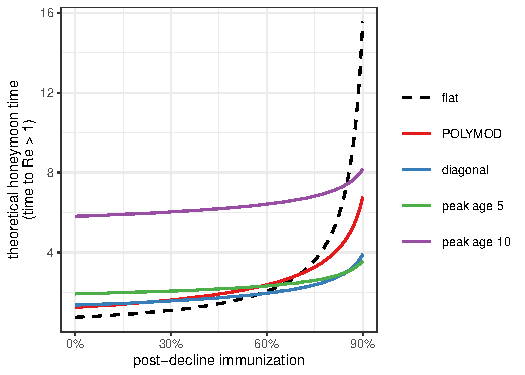
\includegraphics[width=0.8\textwidth]{../figures/honeymoon_age_full_start95.pdf}
\caption{\textbf{Theoretical honeymoon time predictions under five assumptions about age-structured mixing.} Theoretical honeymoon time, computed as time until $\Reff>1$, by vaccination levels after a drop in immunization. Results are shown for a population with $\mu = 1/80$ years\textsuperscript{-1}, a pathogen with $\Rn = 17$, and a pre-decline immunization of 95\%. See Figure S2 for results under higher pre-decline immunization levels.}
\label{fig:age-structured-honeymoon}
\end{figure}

\section{Reported coverage as a lens into the landscape of susceptibility}
\label{sec:reported-coverage}

The above theory invites us to ask how close we may be to these theoretical thresholds, and reported vaccination coverage data can serve as one lens into the timing and magnitude of declines across geographic locations. Here, we analyzed World Health Organization and United Nations Children's Fund (WUENIC) estimates of national immunization levels of measles containing vaccine (MCV1 coverage) from 2000-2023 \citep{WHO_UNICEF2024} and data on measles mumps and rubella vaccine coverage in school age children across US counties since the 2017-2018 school year where data is available \citep{DongEtAl2025}.

We classified each location based on the largest decline in vaccine coverage over consecutive years (Figure \ref{fig:empirical-declines}A-D). Small declines were the most common, with the largest consecutive decline being less than a 6\% drop in 38\% of countries and 63\% of US counties for which we have data. Some locations (e.g., Samoa) saw dramatic, short-term drops, while others saw gradual but sustained declines (e.g., Benin). Yet, in general, the long-term sustained declines that are predicted to be necessary for rebound outbreaks were rarely reported. Under the very coarse assumptions of $\Rn = 17$, a birth rate of $\mu = 1/80$ years\textsuperscript{-1}, pre-decline immunization of 95\% and POLYMOD mixing (dotted line, Figure \ref{fig:empirical-declines}C-D), 10\% of countries (19/190) and 1\% of US counties (20/1999) are predicted to have exceeded their honeymoon times. Even some of these counties may not yet have exceeded theoretical honeymoon times, as this dotted line assumes a constant and sustained drop in immunization (whereas the data often indicate gradual declines).

Our epidemiological theory also predicts that birth rates will modulate the effects of immunization drops on theoretical honeymoon times; both lower levels of immunization and higher birth rates should lead to faster accumulation of susceptible individuals. For this reason, we explored how US county-level birth rates and vaccination coverage correlated with measles outbreaks that have been reported between January 1 2025 and February 13 2026 \citep{JHUMeaslesTracking2026}. Vaccination data was unavailable in 13 states, which collectively reported 160 of the total 3098 measles cases (8\%) during this period. We excluded an additional 90 measles cases (3\%) where the county could not be identified (Table S1). Together, we had vaccination and birth rate data for 2155 counties, of which 215 reported at least one measles case.

Of the 22 county-level outbreaks that comprised the top 10\% in terms of cases per 10,000 population (ranging from 5 to 192), 19 (89\%) had birth rates above average and 10 (45\%) had vaccination coverage below average. There were 8 counties (36\%) that had both higher than average birth rates and lower than average vaccination coverage. There was one county, Borden Texas, which had below average birth rates (76 births per 10,000 vs. an average of 110) and above average vaccination coverage (95.8\% vs. an average of 92.3\%); this county reported 1 case among a population of 654 people (which is equivalent to 15.3 cases per 10,000).

There are also many counties in the empirical data that do not conform to theoretical expectations. For example, average reported vaccination coverage is above 95\% in 74 of the 215 counties (34\%) with at least one measles case. The average number of reported cases among this group is 4.51 (or 1.05 per 10,000, with a range of 1-61 cases or \textless1-15.3 per 10,000). Counties with at least one reported case despite high coverage highlight the possibility for infections among susceptible individuals, even when surrounded by otherwise vaccinated populations. The coarse reported coverage metric used here also likely misrepresents true population-level susceptibility.

On the other hand, there are a number of counties with low coverage (and in some cases high birth rates) that have not reported any measles cases. Of the 2155 counties for which we have birth rate and vaccination data, 901 (42\%) have coverage between 90\% and 95\% and an additional 462 (21\%) have coverage below 90\%. In counties with coverage below 90\%, only 38 (8\%) have reported at least one measles case. These could be places where imported infections may not yet have seeded outbreaks, highlighting the role of connectivity and importation.

As a preliminary exploration of how likely it is that importations have not yet seeded outbreaks in many places, we extended our honeymoon theory to a simple metapopulation model where patches are equally connected and some percentage of patches experience a drop in immunization (the others remain at pre-decline immunization levels). In this case, a small degree of connectivity can increase honeymoon times, where the low immunization patches are effectively buffered by those that have not dropped Figure S3). If patches are connected such that 1\% of transmission is shared between them, honeymoon times increase by 6\%-9\% (35\%-37\% increases with 5\% shared transmission, and 70\%-76\% with 10\% shared transmission). Such dynamics could further delay outbreaks.

\begin{figure}[p]
\centering
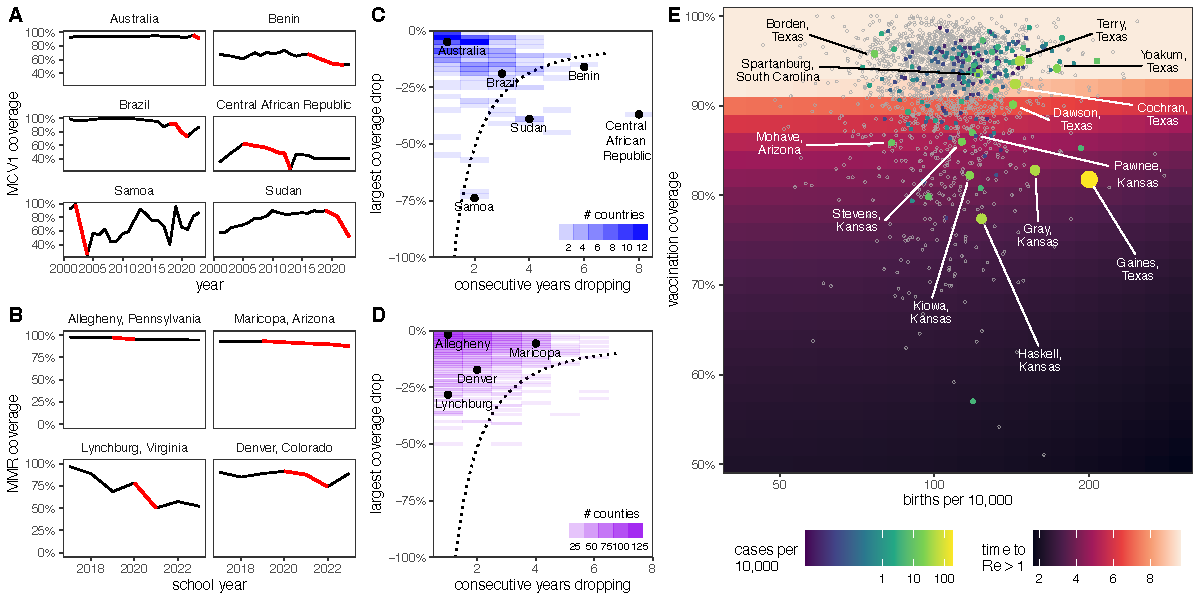
\includegraphics[width=\textwidth]{../figures/empirical_vax_declines_v3_AI.pdf}
\caption{\textbf{Interpreting observed vaccination coverage declines.} (A) First dose coverage of measles containing vaccine (MCV1) in six example countries, and (B) coverage of measles mumps and rubella vaccination in four example US counties. In both, consecutive declines in coverage are shown in red. (C-D) Heatmap of coverage declines in WHO countries (C) and US counties (D), where locations are classified based on the largest drop in vaccination coverage and the number of consecutive years over which the drop occurred. Sample locations are highlighted with points, and the theoretical honeymoon threshold is shown for reference when $\mu = 1/80$ years\textsuperscript{-1}, $\Rn = 17$, pre-decline immunization = 95\% and age-structured contacts follow the POLYMOD mixing matrix. (E) US counties classified by birth rate and average vaccination coverage from 2017-2024 (where data is available). Colored points represent counties with at least one measles case; the color and size of the point show cumulative cases per 10,000 population since January 1, 2025 on the log scale. Counties with no reported measles cases (and available vaccination data) are shown with open gray circles. For reference, the background heatmap shows theoretical honeymoon time predictions under the same assumptions as (C-D); contours highlight theoretical honeymoon times of 3, 5, and 7 years. Counties with the top 5\% of outbreaks (in terms of cumulative cases per 10,000 population) are labeled. WUENIC data on national immunization levels for MCV1 from \citep{WHO_UNICEF2024}, US county level MMR data from \citep{DongEtAl2025}, measles outbreak data from \citep{JHUMeaslesTracking2026}, and county level birth rates from US Census Bureau \citep{SocialExplorer2019}; see Methods for additional details about data and analysis. 10 counties with birth rates below 40 per 10,000 are not shown; there were no reported measles cases in these counties.}
\label{fig:empirical-declines}
\end{figure}

\section{Discussion}
\label{sec:discussion}

Declines in childhood vaccination coverage are an increasingly pervasive problem, leading to questions about the impending return of vaccine preventable diseases. The concept of an epidemiological honeymoon, or a period with minimal transmission despite sub-optimal control, is an important tool for understanding outbreak risk in this scenario. Like much of epidemiological theory, honeymoons have been understood in the context of increasing vaccination coverage, but here we recontextualize this theory to address honeymoon periods under declining vaccination.

The key pillar of our theoretical analysis is that the re-accumulation of susceptible individuals is typically a slow, gradual process \citep{MetcalfEtAl2020,KiangEtAl2025}. Birth cohorts are small compared to the general population, and are getting smaller as birth rates decline globally \citep{BhattacharjeeEtAl2024}. The pace of fertility decline varies substantially across countries (as well as smaller geographic regions), and these changes will have implications for reemergence patterns going forward \citep{BakerEtAl2022}. Some fraction of each birth cohort also remains protected, as annual drops in coverage tend to be modest. A consequence of this slow accumulation process is that we should anticipate (potentially long) lags between the point at which coverage starts to decline and the outbreaks that will eventually ensue. However, complexities in age-specific contact patterns can shorten these lags and make outbreaks faster than if susceptibles and contacts were evenly distributed throughout the population.

Nevertheless, it is clear that we are now in the midst of vaccination decline; accumulation of susceptibles has been occurring over the past years, and potentially decades. There are already many communities with enough susceptibles to fuel an outbreak \citep{ChenBento2026,ZhouEtAl2026,DongEtAl2025}, and ongoing outbreaks demonstrate the reality of this possibility \citep{DoMulholland2025}.

Our ability to change course on this problem depends on a number of factors. Estimating community-level or school-level susceptibility will be necessary for anticipating where outbreaks may occur and planning response programs, including supplemental vaccination campaigns. Yet, challenges with reporting and vaccination data inhibits our ability to reliably infer susceptibility \citep{ChenBento2026,ZhouEtAl2026,FitzpatrickEtAl2026,MastersEtAl2020,BhatiaEtAl2025}. \textbf{Nuanced serological surveys} that target different populations and age groups (e.g., schools) will be an important tool to independently verify susceptibility estimates \citep{LesslerEtAl2016,WinterEtAl2018,MetcalfEtAl2020}, and may reveal the potential role of waning antibody titers from periods of low circulation \citep{MenezesEtAl2025,RobertEtAl2024,OsmanEtAl2026}. Serological studies become even more important for pathogens with high rates of asymptomatic infection. Potentially most pressing, however, is the need to understand and overcome vaccine hesitancy \citep{HijanoEtAl2025,OliveEtAl2018}.

Additional developments beyond the basic theory we have presented will be necessary going forward. First, we have primarily focused on homogeneous and age-structured populations, but clustering in beliefs, vaccination status and contact patterns among communities shape the landscape on which outbreaks emerge \citep{KlinkenbergEtAl2022,ChenBento2026,MastersEtAl2020,FitzpatrickEtAl2026}. The tools we have used to understand age structure, such as the unity beta calculation, can easily be extended to other types of structured populations. Beyond this theory, more work remains to understand the underlying drivers of these heterogeneities \citep{BauchEarn2004,SalatheBonhoeffer2008,MbahEtAl2012,GarnierEtAl2020,KonstantinouEtAl2021,AlvarezZuzekEtAl2022} as well as their implications for epidemiological outcomes \citep{TrueloveEtAl2019,GromisLiu2021,HarrisEtAl2026}.

The networks by which communities are connected will also be a key driver of post-honeymoon outbreaks \citep{ColizzaEtAl2006,Riley2007}. Our simplest theoretical assumptions suggested that under-vaccinated communities within a broader network of vaccinated places can be effectively buffered from importations and therefore outbreaks. Yet, network structured dynamics will have important nuances that these simple assumptions cannot capture (e.g., network structure can accelerate outbreaks, for example if under-vaccinated communities are more connected to one another). Characterizing the global network on which vaccine preventable disease may spread (including the connectivity of children within and between schools), and \emily{Replace the initial ``i'' in ``identifying'' with ``may shed light on why we have not yet seen measles outbreaks take off across the many undervaccinated communities that exist. I''.}identifying the theoretical point after which network-level immunity is predicted to collapse will be essential going forward. Pathogen sequencing will also be a key tool in this endeavor. Network-level dynamics, however, may be difficult to anticipate as synchrony in outbreaks has been shown to deteriorate with increasing vaccination coverage \citep{LauEtAl2020}.

In addition to our simplifying theoretical assumptions, there are also a number of limitations with the empirical data we have presented. We have taken national and county-level immunization estimates at face value, but there are many biases present and subtleties to interpreting these data, including for example challenges with reporting as well as subnational and local heterogeneities. Moreover, vaccination data is not available for all countries and US states, which likely introduces additional inaccuracies. We have coarsely summarized vaccination coverage over time and only used birth rates from a single year, so we cannot reliably reconstruct susceptibles, as indicated by the mismatch in predicted and observed outbreak risk (Figure 5). However, other careful reconstructions can be used to estimate realistic effective reproduction numbers and honeymoon times to support planning and response \citep{ChenBento2026}. Leveraging pathogen phylodynamics during periods of reemergence is a key area for future work.

Ongoing declines in childhood immunization threaten decades of public health progress. If this trend continues, the reemergence of vaccine preventable disease is inevitable. Our theory suggests that this reemergence process may be slowed by a number of factors. New susceptibles accumulate through births gradually, especially when coverage declines are modest, and under-vaccinated communities are nested within a broader network of vaccinated communities. Age structure can buffer some of these effects, potentially shortening the time to rebound outbreak and making outbreaks more explosive when they do occur. Nevertheless, this theory offers hope that we still have time to respond with our most effective public health intervention, vaccination, and underscores the importance of grappling with major contemporary challenges including vaccine hesitancy.

\section{Methods}
\label{sec:methods}

\subsection{Theoretical honeymoon times}
\label{sec:methods-theoretical-honeymoon}

The observed ``post-honeymoon time'' will depend both on the susceptibility in the population and the frequency and timing of importations \citep{MetcalfEtAl2020}. Here we focused exclusively on the accumulation of susceptibles, defining the theoretical honeymoon time as the time until $\Reff=\Rn S(t)$ crosses 1. We chose this definition because it represents the time after which an importation would successfully lead to an outbreak (deterministically). It also has the advantage of being analytically tractable.

\subsection{SIR model from epidemiological theory}
\label{sec:methods-sir}

We derived theoretical honeymoon times in the simplest case with a basic \textbf{S}usceptible-\textbf{I}nfected-\textbf{R}ecovered model. We assumed a constant population size (i.e., birth rate = death rate), where immunization occurs at birth. Although we did not explicitly include vaccine efficacy, it can be understood as reducing the effective vaccination coverage (for example, 94\% coverage with 95\% efficacy would be equivalent to approximately 90\% immunization in our model). The system of differential equations can be defined as follows:

\begin{align}
\dd{S}{t} &= \mu N(1-v)-\frac{\beta SI}{N}-\mu S, \notag\\ \dd{I}{t} &= \frac{\beta SI}{N}-(\gamma-\mu)I, \notag\\ \dd{R}{t} &= \mu Nv+\gamma I-\mu R.
\label{eq:sir-main-methods}
\end{align}

where $\mu$ is the birth and death rate, $v$ is the proportion of new births that are immunized, $\beta$ is the transmission rate, and $\gamma$ is the recovery rate. Going forward, we assume the total population size, $N$, is 1 and thus our system of differential equations tracks the percent of the population in each class. We can derive the accumulation of susceptible individuals when measles is locally extinct (i.e., when $I = 0$)

\begin{equation}
S(t)=(1-v)+\bigl(S_0-(1-v)\bigr)e^{-\mu t}.
\label{eq:susceptible-main-methods}
\end{equation}

and the time until $\Reff=\Rn S(t)=1$

\begin{equation}
\text{theoretical honeymoon time} =-\frac{1}{\mu}\log\!\left(\frac{1/\Rn-(1-v)}{S_0-(1-v)}\right) =-\frac{1}{\mu}\log\!\left(\frac{S^*-S_v}{S_0-S_v}\right).
\label{eq:honeymoon-time-methods}
\end{equation}

Derivations are provided in the supplementary material.

\subsection{Age-structured SIR model}
\label{sec:methods-age-structured}

We extended the basic SIR model to include age structure, such that we have

\begin{equation}
\text{new infections} =\frac{1}{N}\sum_{j=1}^{A}\theta_{i,j}S_i(t)I_j(t).
\label{eq:age-structured-incidence-methods}
\end{equation}

where $A$ is the number of age classes and $\theta_{i,j}$ is WAIFW (who acquires infection from whom) matrix \citep{GrenfellAnderson1989,AndersonMay1991} that determines transmission rates between susceptible individuals of age i, $S_{i}(t)$, and infected individuals of age j, $I_{j}(t)$. Full model equations are provided in the Supplementary Material. In our simulations, we \hl{defined 4 month age} classes between ages 0 and 15, and 5 year age classes until age 100.

We tested five WAIFW matrices that span a range of contact-heterogeneity possibilities, (1) a \ul{flat} matrix, where contacts are equivalent across all age groups (equivalent to the homogeneous SIR model described in the previous section); (2) an empirically grouped matrix derived from the \ul{POLYMOD} contact surveys \citep{MossongEtAl2008}; and three synthetic matrices where (3) contacts are most intense along the \ul{diagonal} (i.e., among individuals of similar ages), and (4 and 5) where contacts \ul{peak at age 5} or \ul{peak at age 10} and there are minimal contacts among other age groups.

To generate the synthetic contact matrices we followed \citep{FarringtonWhitaker2005}, where contacts between age $x$ and $y$ are defined as $\beta(x,y)\  = \ \gamma(u)b(v|u)$, where $u\  = \frac{x + y}{2}$ and $v\  = \frac{x - y}{2}$. The first component functions is defined as

$\gamma(u;\mu,\ \sigma)\  = c^{- 1}x^{1/\sigma^{2} - 1}e^{- \frac{1/\sigma^{2}u}{\mu}}$

where $c\  = \mu(1 - 1/\sigma^{2}))^{(1/\sigma^{2} - 1)}e^{1 - {1/\sigma}^{2}}$, and the second component function is

$b(v|u;\phi)\  = \frac{(u + v)^{\alpha - 1}(u - v)^{\alpha - 1}}{u^{2\alpha - 2}}$

where $\alpha = \frac{1 - \phi}{2\phi}$. In general, this approach will generate a symmetric matrix with $\mu$ defining the age at which most contacts occur, and $\gamma$ and $\sigma$ define the variance around this point relative to the diagonal and the off-diagonal of the matrix. We used $\mu = 7,\ \sigma = \ 0.6,\ \phi = 0.05$ for the diagonal matrix, $\mu = 5,\ \sigma = \ 0.2,\ \phi = 0.05$ for the peak at age 5 matrix, and $\mu = 10,\ \sigma = \ 0.1,\ \phi = 0.01$ for the peak at age 10 matrix. The contacts in each matrix were scaled such that all matrices yielded a $\Rn$ of 17 (calculated using the next generation matrix method \citep{DiekmannEtAl1990}, see Supplementary Material).

We then simulated the accumulation of susceptible individuals after vaccination declines and calculated the time until $\Reff>1$ using each WAIFW matrix. Again $\Reff$ was calculated using the next generation matrix method. In addition, we used the unity beta calculation \citep{EarnEtAl2000,Mahmud2017,Bjornstad2018} to quantify the extent to which age structure ``slows down'' or ``speeds up'' dynamics relative to the homogeneous SIR model. We derive this by calculating a time-varying equivalence between the age-structured model and the homogeneous model (see Main Text and Supplementary Material for details).

\subsection{Metapopulation model}
\label{sec:methods-metapopulation}

We expanded our model to consider a simple network of equally connected patches. We assume that some percent of patches experience a drop in immunization levels, and the others remain at pre-decline levels; aside from immunization, patches are otherwise identical. We can again track the buildup of susceptible populations in each of these patches, and use the next generation matrix method to calculate the point at which the effective reproduction number exceeds one. Details are provided in the Supplementary Material.

\subsection{Empirical data}
\label{sec:methods-empirical}

We used World Health Organization and United Nations Children's Fund WUENIC national immunization estimates for the first dose of measles containing vaccine (MCV1 coverage) from 2000-2023 \citep{WHO_UNICEF2024}. This included 195 countries, and we excluded 3 that did not have complete reported coverage data (South Sudan, Montenegro, Timor-Leste). Methodological details can be found in \citep{BurtonEtAl2009}

At the US county level, we used data compiled by \citep{DongEtAl2025} on county-level coverage of measles mumps and rubella vaccination (MMR) since the 2017-2018 school year, comprising 2237 counties across all states except Alaska, Arkansas, Delaware, Georgia, Idaho, Illinois, Indiana, Mississippi, Montana, Nebraska, New Hampshire, Ohio and West Virginia.

We downloaded US Census data on county-level births and population size from Social Explorer \citep{AlvarezZuzekEtAl2022}. We used the most recent data that was available for all counties, which was from 2019.

Finally, we used the Johns Hopkins University Measles Tracking Team data to characterize US county-level reported measles cases. As described in the main text, states without vaccination data were excluded, and cases that were not associated with a specific county were also excluded. In some states, cases were reported at a regional level. In these cases, we used internet sources to map counties in a state to each health region; we then calculated population-weighted averages of vaccination coverage and birth rates for each region. Details on this process and all exclusions are included in Table S1.

\section*{Acknowledgements}

We thank Matt Ferrari for helpful comments on empirical data analysis, and Princeton University librarians Maria Kochis and Ofira Schwartz-Soicher for their assistance obtaining demographic data. EH, BG, and CJEM have been funded in whole or in part with Federal funds from the National Cancer Institute, National Institutes of Health, under Prime Contract No. 75N91019D00024, Task Order No. 75N91023F00016. The content of this publication does not necessarily reflect the views or policies of the National Institutes of Health or the Department of Health and Human Services, nor does mention of trade names, commercial products or organizations imply endorsement by the U.S. Government. BTG and CJEM also acknowledge support from Princeton Catalysis and Princeton Precision Health. This material is also based upon work supported by the High Meadows Environmental Institute at Princeton University.

\section*{Data and code availability}

All data and code used to generate this manuscript are available at \url{https://github.com/eahowerton/measles-honeymoon} and archived at \hl{ADD ZENODO HERE}. 


\begingroup
\small
\bibliographystyle{measles_honeymoon}
\bibliography{measles_honeymoon}
\endgroup

\end{document}
